\documentclass[a4paper,11pt]{article}
\usepackage[top = 1.5 in, bottom = 1 in, left = 1 in, right = 1 in]{geometry}
\usepackage[utf8]{inputenc}
\usepackage[T1]{fontenc}
\usepackage{csquotes}
\usepackage[british]{babel}
\usepackage{lmodern}
\usepackage{url}
\usepackage{color}
\usepackage{graphicx}
\usepackage{setspace}
\usepackage{pdfpages}

\begin{document}
\title{Course project: Mini-PL interpreter}
\author{Laura Leppänen \\ Student number: 013302782 \\ Compilers, Spring 2012}
\date{\today}
\maketitle
\thispagestyle{empty}

\tableofcontents
\onehalfspacing

\newpage
\setcounter{page}{1}

\section{Interpreter implementation}

This section covers the general architecture of the interpreter, testing, error handling as well as building and running instuctions.

\subsection{Architecture}

\begin{figure}
    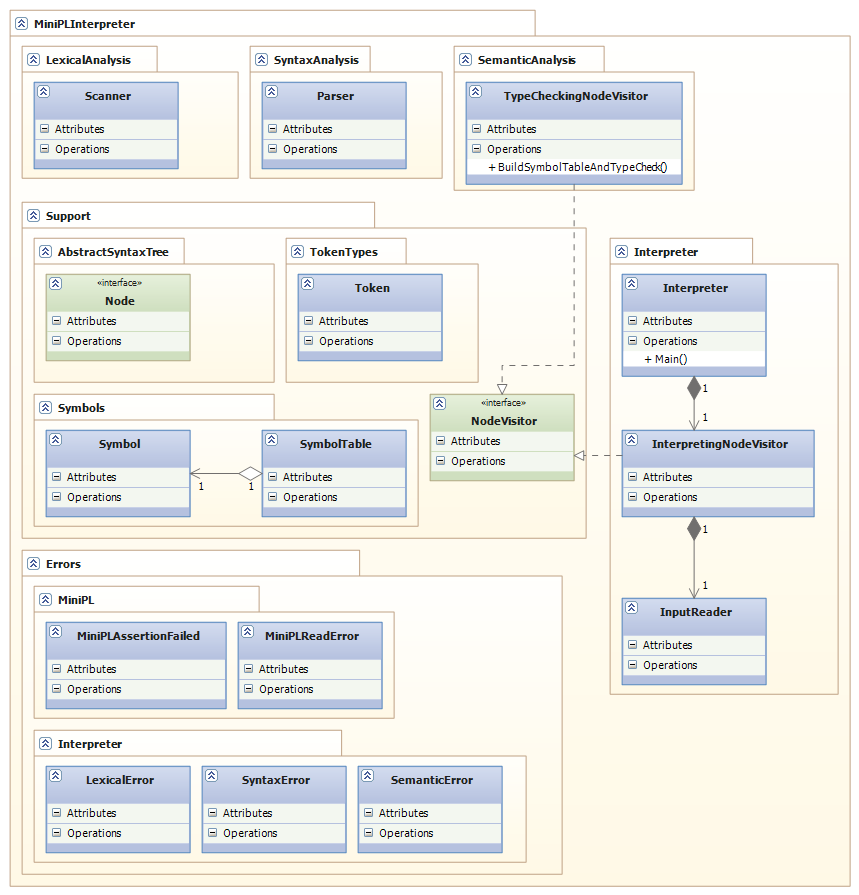
\includegraphics[scale=0.7]{architecture.png}
    \caption{The architecture of the interpreter exluding different token and node classes and package imports to maintain clarity. See the abstract syntax tree description for a list and a diagram of Node classes. Token classes roughly correspond to Node types in AbstractSyntaxTree.}
    \label{fig:architecture}
\end{figure}

Figure \ref{fig:architecture} shows the general architecture of the program. Package (or namespace) imports have been excluded to maintain clarity. Lexical analysis (the Scanner class), syntax analysis (the Parser class), semantic analysis (the TypeCheckingNodeVisitor class) and interpretation (everything in the Interpreter namespace) are architecturally completely separate.

In practice, the Parser needs to be given a Scanner instance that it can call for new tokens as a parameter. My Scanner implementation does not evaluate the whole source code at once but matches and returns one token at a time when NextToken() is called, so in practice lexical analysis and syntax analysis are interleaved. If desired, however, this could trivially be changed so that Scanner builds e.g. a queue of tokens in one pass of the source code, returning them one at a time on calls to NextToken(), but I did not see a reason for it. The only peculiarity this may cause is that sometimes a syntax error may be detected before a lexical one. Parser is, of course, oblivious to how the Scanner works internally, as long as NextToken() always returns a valid Token object.

The Parser produces an abstract syntax tree. The abstract syntax tree is then traversed by the TypeCheckingNodeVisitor that produces a symbol table. In addition to producing the symbol table it checks for static type errors as well as that variables are declared before use but not declared more than once. The symbol table is then given to the InterpretingNodeVisitor that also traverses the abstract syntax tree and executes the commands described by it. The Main() function in the Interpreter class coordinates the correct order of execution.

The Interpreter namespace also contains an InputReader class for buffered reading of input in executing Mini-PL read statements. Buffered reading is required because the Mini-PL specification (see appendix) requires that reading be done one whitespace-delimited word at a time whereas C$\sharp$ only provides reading one character at a time or one line at a time. The InputReader is in the Interpreter namespace mostly because other modules do not use it.

Utilities that are used by several different packages or namespaces are in the Support namespace. These include AbstractSyntaxTree (used in parsing, semantic analysis and interpretation), TokenTypes (used by Scanner and Parser), Symbol (containing Symbols and SymbolTables, used in semantic analysis and interpretation) and the NodeVisitor interface, implemented by InterpretingNodeVisitor and TypeCheckingNodeVisitor.

Errors have their own namespace which is in turn divided into interpreter errors (lexical, syntactic and semantic) and Mini-PL errors. These are described in the error handling section below.

I have attempted to name variables, classes and functions and structure the code in such a way that minimal comments are required to follow it. Sometimes I have included implementation notes explaining my choices or references to more abstract constructs (such as the CFG) in comments.

\subsection{Error handling}

As described in the architecture section, the Errors namespace is divided into interpreter related errors that can be lexical, syntactic or semantic, and Mini-PL related exceptions.

LexicalErrors are thrown by the Scanner, SyntaxErrors by Parser and SemanticErrors by TypeCheckingNodeVisitor. The types of semantic errors reported are type mismatch, integer overflow in an integer literal, reference to an unknown variable and declaration of a variable that is already defined. Whenever possible, error messages contain row and/or column information and possible additional information about the offending token. When both a row and a column are specified in the message, the actual language token referenced resides immediately before that point in the source code. Both row and column numbering start from 1.

It should be noted that my implementation raises a SemanticError if for loop bodies contain variable declarations. Because everything in Mini-PL programs resides inside a single scope (as specified in the Mini-PL specification, see appendix), a variable declaration in a for loop that has more than one iteration causes that variable to be declared several times, which is not allowed. Of course a for loop that is iterated over only once would not cause this problem but since for loops that iterate over the body less than twice make little sense, I decided to disallow variable declarations inside loop bodies altogether. Of course more sensible and slightly more complex scoping rules would have the for loop create its own scope ''inside'' the scope of the main program but that goes against the specification.

Out of the Mini-PL exceptions, only assertion failure is mentioned in the specification. InterpretingNodeVisitor throws MiniPLAssertionFailed when a Mini-PL assert statement fails (the argument to assert is false). To handle errors encountered in reading integers when executing a read statement, MiniPLReadError is introduced. It is thrown when a read statement attempts to read an integer and either the input is not a valid integer or an integer overflow occurs when converting to a 32-bit signed integer.

All errors (both Interpreter and Mini-PL) are handled by a try-catch statement wrapping most of the body of the Main() function in the Interpreter class. When an exception is raised, the Main() function prints the error message and exits. The interpreter does not utilize any error recovery strategies for reporting possible multiple errors in a source file at a time, but this did not appear to be a requirement judging by the project specification.

\subsection{Testing}

The project MiniPLInterpreterTest, included in the \verb,src, directory contains unit tests for most of the source code. Tests were written using NUnit\footnote{\url{http://www.nunit.org}} 2.6 and run using TestDriven.Net\footnote{\url{http://testdriven.net}} (Personal, version 3.3.2779 Beta 2). The scanner was developed in a test driven manner. The parser and visitors were developed by writing a complete rudimentary version first and then writing tests for all distinct cases I managed to think of to guide further development and to find bugs. Each phase was (unit) tested separately, though I trusted my Scanner implementation enough to use it in my Parser tests (of course some kind of a scanner stub for testing would have been a more sound way to perform these tests). Currently all unit tests pass.

I did not have enough time to do proper integration testing, so I just ran a few small programs as a form of non-automated ad-hoc integration testing and fixed the bugs that I found by first adding a new failing unit test and then making it pass. Some test programs were valid, some contained errors, so I could see error handling in action, and some tested functionality that I was more or less suspicious of. These programs included the example programs given in the Mini-PL specification (see appendix). All bugs that I managed to find were fixed.

\subsection{Building and running the interpreter}

On Windows, open the solution file (\verb,MiniPLInterpreter.sln,) in Visual Studio. The CS department winserver appears to have Visual Studio 2010 Professional which does not support UML modeling projects such as the InterpreterUML project which contains the architecture diagram. Hence, upon opening the solution, Visual Studio will show an error message. The other projects, however, will be loaded properly. The UML project will also work fine on Visual Studio 2010 Ultimate.

If NUnit is missing (like on the CS department winserver) or is an older version, building the whole solution will fail, so in that case choose only the main project (MiniPLInterpreter) and choose ''build MiniPLInterpreter`` from the build menu. This produces an executable file in the \verb,bin, directory under \verb,MiniPLInterpreter,.

The interpreter does not provide a REPL, so to run a program the source code file must be given as a command line parameter:

\begin{verbatim}
$ MiniPLInterpreter.exe path\to\program.mpl
\end{verbatim}

\newpage
\section{The Mini-PL language}

This section covers issues related to scanning and parsing Mini-PL: token patterns, the context-free grammar, and the abstract syntax tree.

\subsection{Mini-PL token patterns}

\begin{table}[h!]
\begin{tabular}{| l | l |}
    \hline
    Token type & Regular expression \\
    \hline
    Variable or keyword \textsuperscript{1} & [a-zA-Z][0-9a-zA-Z]* \\
    \hline
    Integer literal & [0-9][0-9]* \\
    \hline
    String literal \textsuperscript{2} & "([\^{}"\textbackslash]|(\textbackslash[\textbackslash tnrv"]))*" \\
    \hline
    Endline symbol & ; \\
    \hline
    Assignment symbol & := \\
    \hline
    Colon symbol (type declaration) & : \\
    \hline
    Operator symbols \textsuperscript{3} & +|-|*|<|/|=|\&|! \\
    \hline
    Parentheses & (|) \\
    \hline
    Range operator & .. \\
    \hline
\end{tabular}
\end{table}

Notes:
\begin{enumerate}
\item Matching patterns are identified as keywords or variables by checking a predefined keyword list.
\item String literals can contain any characters except non-escaped quotes or backslashes. Valid escape characters are \verb \\ , \verb \n , \verb \t , \verb \v , \verb \r , \verb \" . Note that backslash characters in the regex are character literals with no special escape meaning.
\item The specification (see appendices) lists \verb,!, as a binary operator as well as a unary operator. Because the specification did not specify the meaning of \verb,!, as a binary operator, I assumed it was mistakenly listed as such and only accepted it as a unary operator. The division operator symbol / is special because it can also begin a comment.
\end{enumerate}

Non-token patterns (Note: Here the \textbackslash{} symbol starts an escape character):
\begin{table}[h!]
\begin{tabular}{| l | l |}
    \hline
    Whitespace & (\textbackslash t|\textbackslash r|\textbackslash n|\textbackslash v| )* \\
    \hline
    Single line comment & //[\^{}\textbackslash n]*\textbackslash n \\
    \hline
    Multiline comment & /\textbackslash *.*\textbackslash */ \\
    \hline
\end{tabular}
\end{table}

\subsection{Context-free grammar}

Refer to appendices for the original non-LL(1) grammar. I have renamed \verb,<stmts>, to \verb,<stmt-list>,. \verb,\epsilon, denotes the empty string.

\newpage

\begin{verbatim}
<prog>           ::= <stmt-list>
<stmt-list>      ::= <stmt> ";" <stmt-list-tail>
<stmt-list-tail> ::= <stmt-list>
                  | \epsilon
<stmt>           ::= "var" <var-ident> ":" <type> <opt-assignment>
                  |  <var-ident> ":=" <expr>
                  |  "for" <var_ident> "in" <expr> ".." <expr>
                     "do" <stmt-list> "end" "for"
                  |  "read" <var-ident>
                  |  "print" <expr>
                  |  "assert" "(" <expr> ")"
<opt-assignment> ::= ":=" <expr>
                  |  \epsilon
<expr>           ::= <opnd> <expr-tail>
                  |  <unary-op> <opnd>
<expr-tail>      ::= <op> <opnd>
                  |  \epsilon
<opnd>           ::= <int>
                  |  <string>
                  |  <var-ident>
                  |  "(" <expr> ")"
<type>           ::= "int" | "string" | "bool"
<var-ident>      ::= <ident>
\end{verbatim}

\subsection{Abstract syntax trees}

Figure \ref{fig:ast} (as generated by Visual Studio) shows the basic class structure of my abstract syntax tree implementation. I have tried to differentiate between different types of expressions and statements quite a lot to minimize the need for e.g. operator symbol checks in type checking and interpretation phases and to make it easier to perceive possible faults in parsing code. The basic ideas are the following:

\begin{itemize}
    \item All node classes implement the Node interface that specifies an accept function for NodeVisitors.
    \item \verb,Program, is a Node class that holds a list of \verb,Statements,. All other nodes are \verb,SyntaxElements,.
    \item \verb,SyntaxElements, can be \verb,Statements, or \verb,Expressions,. (A special case is \verb,Range, which is neither because it only appears in a very specific context, in for loop declarations.) Whether a node is a \verb,Statement, or \verb,Expression, decides where it can appear (e.g. an arithmetic operator's operands must be \verb,Expressions,, never \verb,Statements,).
    \item \verb,VariableDeclaration, (which is a \verb,Statement, because it can appear on its own) and \verb,VariableReference, (which is an \verb,Expression,) implement the interface \verb,Variable, which appears as the left-hand side of an assignment operation.
\end{itemize}

\begin{figure}
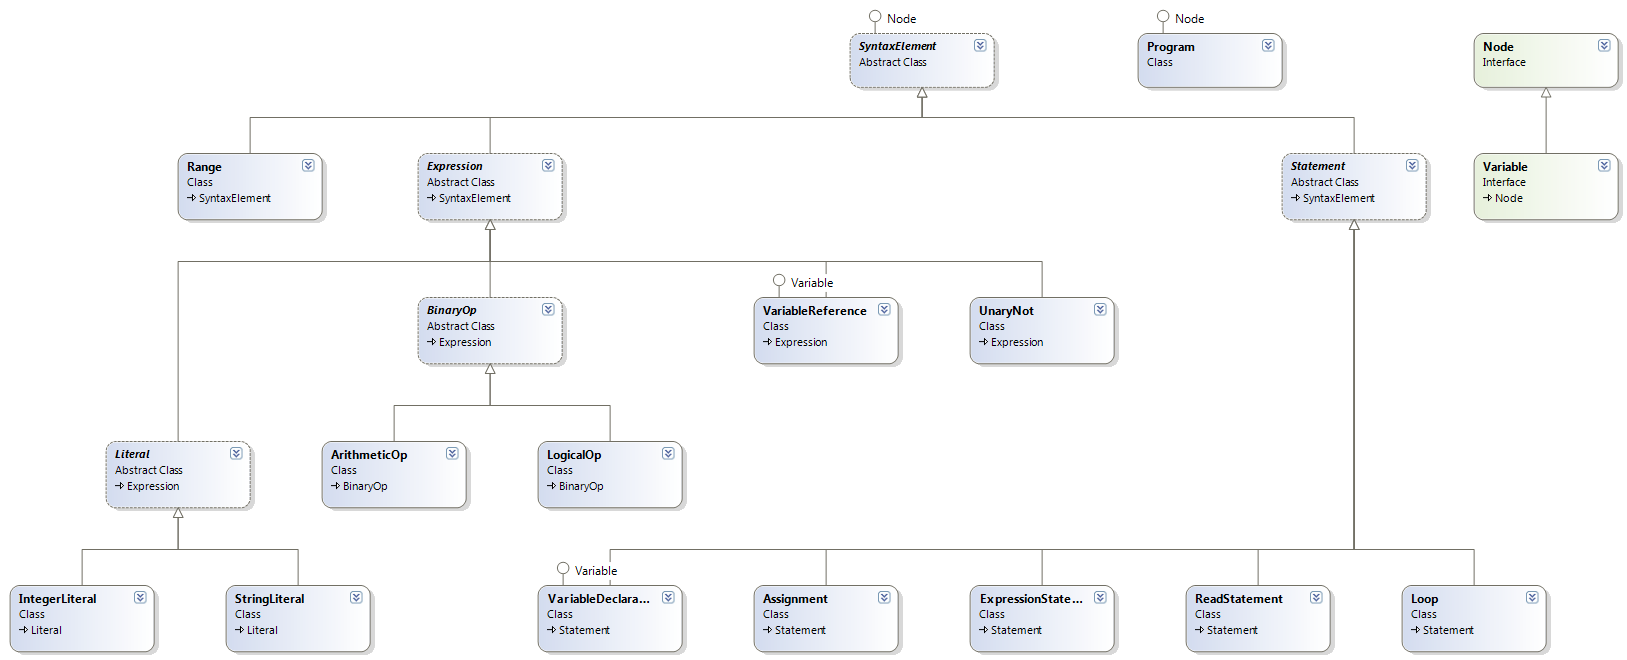
\includegraphics[scale=0.5,angle=90]{ast.png}
\caption{Node classes and interfaces in the abstract syntax tree}
\label{fig:ast}
\end{figure}

The following is a list of different Node constructors\footnote{All constructors additionally take a source row number as a parameter for use in error messages, but I have left these out for clarity} with inheritance information:
\begin{itemize}
    \item \verb,Program(List<Statement> statements),
    \item \verb,IntegerLiteral(string value), (is a \verb,Literal, which is an \verb,Expression,)
    \item \verb,StringLiteral(string value), (is a \verb,Literal, which is an \verb,Expression,)
    \item \verb,VariableReference(string name), (is an \verb,Expression, and a \verb,Variable,)
    \item \verb/ArithmeticOp(string opsymbol, Expression lhs, Expression rhs)/ (is a \verb,BinaryOp, which is an \verb,Expression,)
    \item \verb/LogicalOp(string opsymbol, Expression lhs, Expression rhs)/ (is a \verb,BinaryOp, which is an \verb,Expression,)
    \item \verb/UnaryNot(Expression operand)/ (is an \verb,Expression,)
    \item \verb/Range(Expression lhs, Expression rhs)/
    \item \verb/VariableDeclaration(string name, string type)/ (is a \verb,Statement, and a \verb,Variable,)
    \item \verb/Assignment(Variable variable, Expression expression)/ (is a \verb,Statement,)
    \item \verb/ExpressionStatement(string keyword, Expression expression)/ \footnote{ExpressionStatement covers those statements that begin with a keyword and take an expression as a parameter. In practice, this means assert and print. The read statement is more specific: it only accepts a VariableReference.} (is a \verb,Statement,)
    \item \verb/ReadStatement(VariableReference variable)/ (is a \verb,Statement,)
    \item \verb/Loop(VariableReference variable, Range range, List<Statement> body)/ (is a \verb,Statement,)
\end{itemize}

\appendix
\section{Appendices}

Start on page 9 after figure \ref{fig:ast}. Includes project specification and Mini-PL specification.

\includepdf[pages={1, 2}]{project_spec.pdf}

\includepdf[pages={1, 2, 3}]{minipl_spec.pdf}

\end{document}
